%\section{Geometrical indicator for voltage unbalance in three phase networks.}

\section{Network structure}

%        \textcolor{magenta}{MACI}\\
         The examined network is supposed to be the low voltage local transformer area with regular households, depicted in Figure \ref{fig:network}. \textcolor{magenta}{The network structure of Figure \ref{fig:network} has been implemented in Simulink\texttrademark\, environment for simulation based experiments}. Most of the households represent a single phase load \textcolor{magenta}{with resistive inductive and capacitive properties} while some of them are \textcolor{magenta}{symmetric} three phase ones. There might also be some households with domestic powerplant, they are not only loads but also
         represents distributed generators. \textcolor{magenta}{Furthermore, it is assumed that the households located on a domestic size grid tie inverter are also provided with battery storage capacities.} Commercially available inverters are capable of optimizing the working point and charging current of the system, while the ability of power quality improvement is far not typical - it is in experimental phase in some cases, e.g. \cite{gorbe2012reduction}.%

        \begin{figure}[!ht]
            \centering
            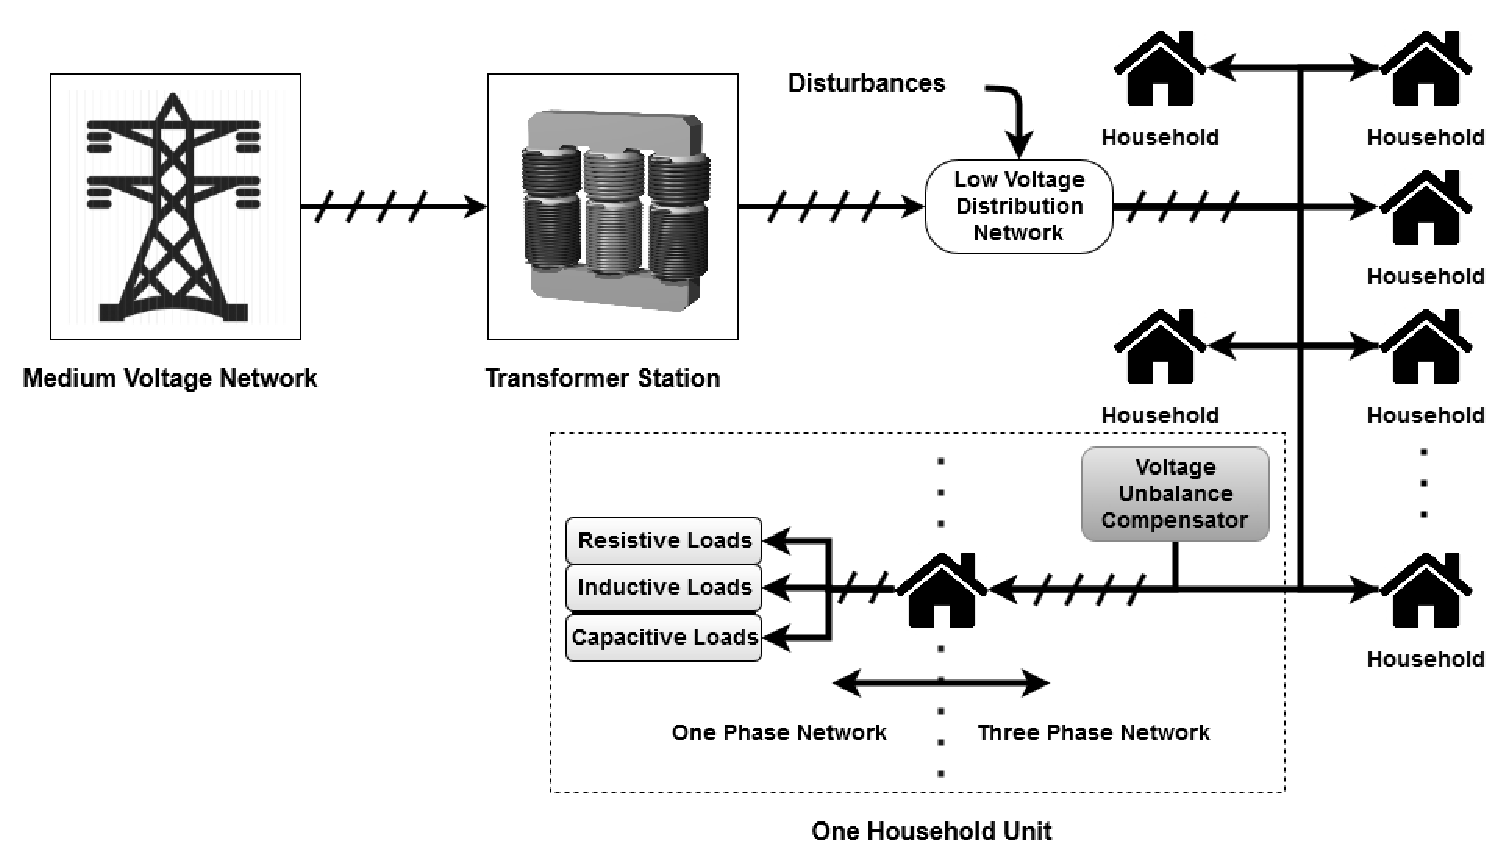
\includegraphics[width=\textwidth]{Unblance_EPS_Pics/network_gray.eps}
            \caption{The simplified structure of a three phase four wire low voltage network. The transformer station acts as transition from the medium voltage power grid to
            the low voltage network. The several regular households are representing the main loads of the network. The transformer and the loads are connected with power line sections infected by inductive and resistive disturbances and capacitive couplings. Domestic powerplants can connect to any connection point within the low voltage network, via an appropriate inverter - either to the three phase sections using a three phase inverter or to a single phase using a single phase inverter.}
            \label{fig:network}
            \end{figure}


    \section{Voltage deviations}


        \textcolor{red}{The paper focuses on three types of voltage deviations. The first fall in to the category of unbalance, namely any kind of phase deviations, and unbalanced amplitude deviations, and balanced amplitude deviations, like under-voltage.} There are many different technological causes with more or less practical importance. The following conditions are examined and tested in the sequel:
        \begin{description}
        \item[Single phase under-voltage unbalance]  If there is a single phase uncompensated overload in the system, the voltage in the overloaded phase will be lower than the other two.
        \item[Two phase under-voltage unbalance]  Two of the three phases are overloaded without compensation, the two overloaded phases will have higher voltage drop than the third phase.
        Balanced three phase under-voltage]  The loads of all three phases are overloaded in an unbalanced manner.
        \item[Unbalanced single phase angle]  If the three phase voltage amplitudes are balanced but the relative angles between them (ideally it should be equal to $\pm120$ degree). It is assumed, that phase A would be the reference. If one of the other two phase angles is deflected, unequal displacement.
        \item[Unbalanced two phase angles displacement] Similar to the single phase angle unbalance, if the other two phase angles are both deflected, then unequal angle displacement in two phase angles occurs.
        \end{description}
        An indicator of the voltage unbalance is supposed to measure the extent of unbalance but it is not expected to classify between the above types.

        

        \subsection{Proposed geometrical indicator}

            It can be stated that every difference between the ideal and the measured voltage in both amplitude phase and sub-harmonics causing a form of \textcolor{red}{voltage deviation}. The problem can also be investigated from a geometrical point of view as it is depicted in Figure \ref{fig:threephase}. The three-phase voltage system's phasor diagram contains three  phase-to-neutral voltage vectors which can be regarded as the points of a triangle (similarly, the three line-to-line vectors can play the role of the edges of the triangle). The two triangles (i.e. the ideal and the actual ones) always intersect except from very extreme and physically meaningless cases. The area where the two triangles do not cover each other (i.e. the difference of their union and intersection) can be used as a norm of voltage \textcolor{red}{quality}. In fact it is computationally more demanding compared to the previous methods, but takes every deviation into consideration \cite{Neukirchner2015},\cite{neukirchner2015examination}. The calculation of error is given by (\ref{equ:geom}).

            \begin{equation}
                \begin{array}{rcl}
                       G&=&\textnormal{Area of }(\bigtriangleup_{Ideal}\cup\bigtriangleup_{Real}-\bigtriangleup_{Ideal}\cap\bigtriangleup_{Real}),
                \end{array}
                \label{equ:geom}
            \end{equation}

            $\bigtriangleup_{Ideal}$ indicates the triangle spanned by the ideal voltage vectors and $\bigtriangleup_{Real}$ the triangle of real voltage vectors. Difference of the ideal and the real triangle's union and intersection defines the norm $G$. \textcolor{olive}{Basically, the algorithm calculates the symmetrical difference of the triangles, stretched from three phase ideal and real voltage vectors.}

            \begin{figure}[!ht]
           \centering
           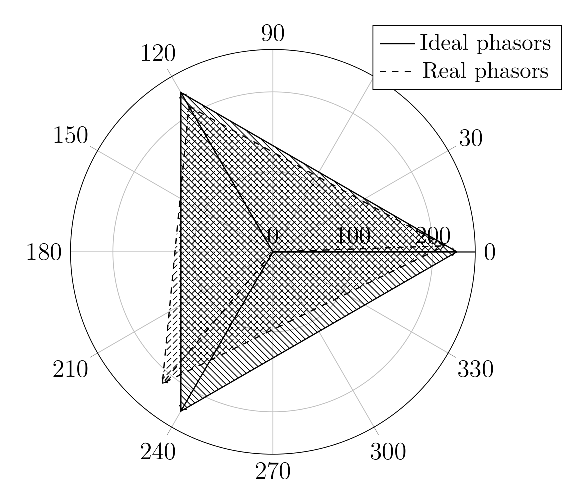
\includegraphics[scale=0.95]{Unblance_EPS_Pics/UnbalRedComp_JCP-figure1.eps}
           \caption{The triangles spanned by the ideal and the actual voltage phasors. The extent of voltage deviation on the network can be measured by the sum of areas where the two triangles are not overlapping.}
           \label{fig:threephase}
            \end{figure}

            \subsubsection{\textcolor{red}{The geometrical method's additional content compared to the regulated method}}

            \textcolor{red}{When using a new method for calculation and cost function it is reasonable to test it's usability against the prevalent or regulated method. In this case the geometrical norm's utility (\ref{equ:geom}) against the TDV (\ref{equ:regular}) value. }
            The geometrical norm was validated experimentally, by investigating the correlation between the regulated (\ref{equ:regular})  and geometrical (\ref{equ:geom}) norms subjected to random, uniformly distributed unbalance on the voltage vector amplitude and phase values with $20$ V amplitude and $1/300\cdot\pi$ rad phase variance (Fig. \ref{fig:correlation}, and Fig. \ref{fig:side_correlation}).

            \begin{figure}[!ht]
           \centering
           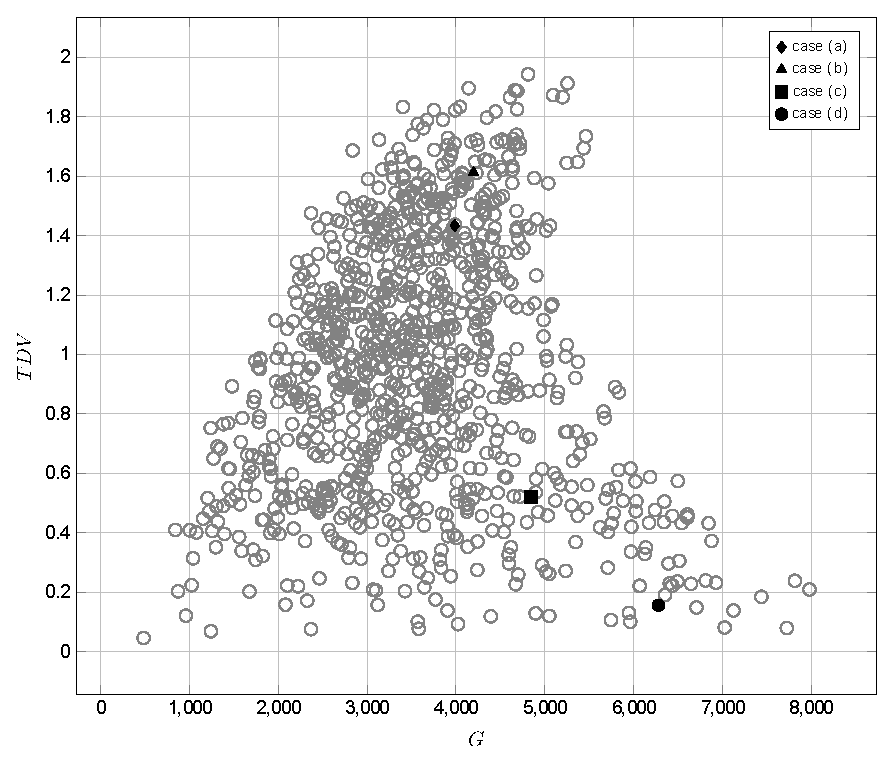
\includegraphics[width=\textwidth,scale=0.95]{Unblance_EPS_Pics/EPS_images/scatter.eps}
           \caption{Correlation between the geometrical voltage unbalance indicator $G$ and the regulated voltage unbalance indicator $TDV$ using 1000 samples. In every iteration each three phase voltage vector's amplitude and phase values changed randomly, according to uniform distributions with $\pm20$ V and $\pm\frac{1}{3}\pi\cdot10^{-2}$ rad variance. It can be seen, that the geometric norm contains more information than the classical one. \textcolor{olive}{The  four asymmetry cases of Figure \ref{fig:cases} are denoted by black symbols on the picture. It is apparent, that in case (c), and (d) the G norm holds additional information than the TDV.}}
           \label{fig:correlation}
            \end{figure}

            \begin{figure}[!ht]
           \centering
           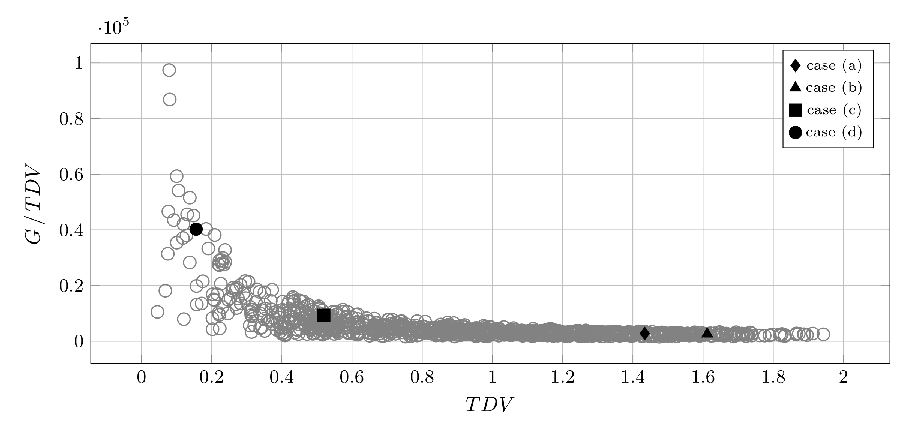
\includegraphics[width=\textwidth,scale=0.95]{Unblance_EPS_Pics/EPS_images/side_scatter.eps}
           \caption{\textcolor{red}{\textbf{Itt a .eps converzio nem lett valami jo, javitani kell!} Correlation between the regulated unbalance indicator and the fraction of geometrical and regulated indicator. It can be seen that there is a functional connection between the two values.}}
           \label{fig:side_correlation}
            \end{figure}


            \textcolor{red}{Although there is correlation between the two norm values in the general case, but for some situations the regular method indicates low, while geometrical norm still indicates high value.\\
            On Figure \ref{fig:cases_A} dominant phase deviation can be observed, while Figure \ref{fig:cases_B} shows amplitude deviation but with opposite direction. When there is such deviation on the grid both indicators present almost identical results. On \ref{fig:cases_C} there is still observable unbalance (two phase deviate stronger than the third in terms of amplitude), but the correlation is significantly lower. In the last case in the lowest correlation area, amplitude deviation is present, but the deviation direction is identical on all phases (balanced over-voltage or under-voltage)(Figure \ref{fig:cases_D}). The regular method indicates very low values. In this case other methods are utilised in parallel in terms of network diagnostics to detect the under-voltage phenomena.\cite{arn1997under-voltage}.}


            \begin{figure}
                \centering
                \begin{subfigure}[b]{0.48\textwidth}
                    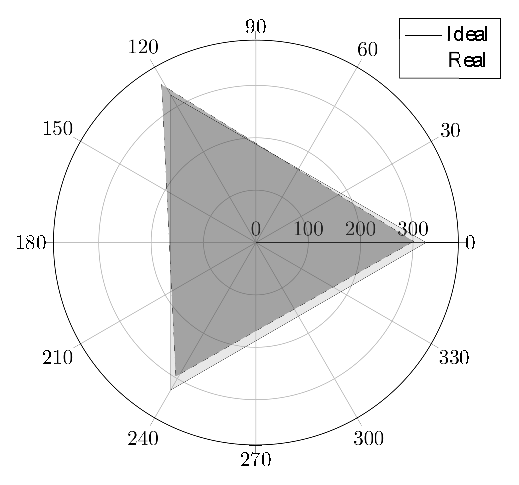
\includegraphics[width=\textwidth]{Unblance_EPS_Pics/EPS_images/rombus.eps}
                    \caption{\centering High correlation with phase deviation. The norm values are $G=3986$ and $TDV=1.434$.}
                    \label{fig:cases_A}
                \end{subfigure}
                ~ %add desired spacing between images, e. g. ~, \quad, \qquad, \hfill etc.
                  %(or a blank line to force the subfigure onto a new line)
                \begin{subfigure}[b]{0.48\textwidth}
                    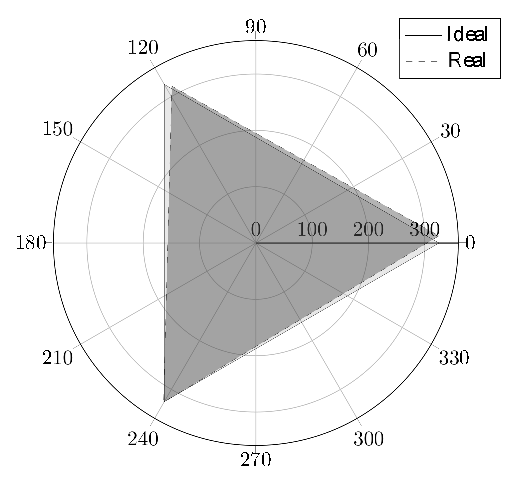
\includegraphics[width=\textwidth]{Unblance_EPS_Pics/EPS_images/triangle.eps}
                    \caption{\centering High correlation with opposed amplitude deviation. The norm values are $G=4198$ and $TDV=1.612$.}
                    \label{fig:cases_B}
                \end{subfigure}
                 %add desired spacing between images, e. g. ~, \quad, \qquad, \hfill etc.
                %(or a blank line to force the subfigure onto a new line)
                \begin{subfigure}[b]{0.48\textwidth}
                    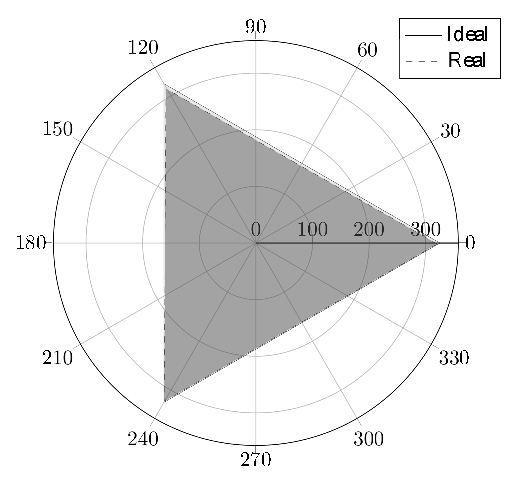
\includegraphics[width=\textwidth]{Unblance_EPS_Pics/EPS_images/square.eps}
                    \caption{Low correlation with opposed amplitude deviation. The norm values are $G=9322$ and $TDV=0.5198$.}
                    \label{fig:cases_C}
                \end{subfigure}
                ~
                \begin{subfigure}[b]{0.48\textwidth}
                    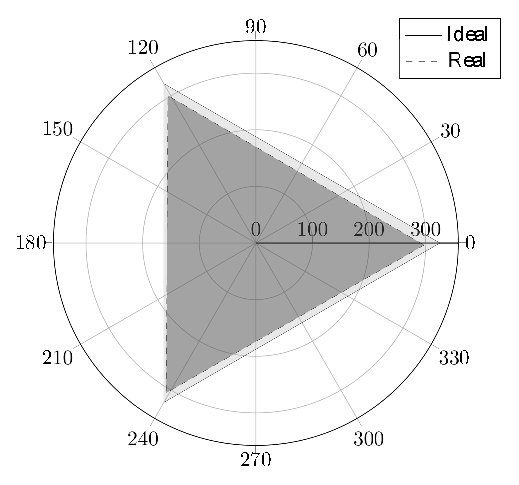
\includegraphics[width=\textwidth]{Unblance_EPS_Pics/EPS_images/circle.eps}
                    \caption{\centering Low correlation with uniform voltage drop. The norm values are $G=6280$ and $TDV=0.156$.}
                    \label{fig:cases_D}
                \end{subfigure}


                \caption{\textcolor{olive}{Four distinct cases of voltage triangles examining correlation between the regular $TDV$ and geometrical $G$ method.}}\label{fig:cases}
            \end{figure}

            \textcolor{olive}{To clarify this, the regular norm's calculation method needs to be investigated. The symmetrical component mutual impedance matrix on a three phase connection point is given by (\ref{equ:mutual}),}

            \begin{equation}
                \begin{array}{rcl}
                       Z_s&=&\frac{1}{3}\begin{bmatrix} 1&1&1\\1&\alpha&\alpha^2\\1&\alpha^2&\alpha \end{bmatrix}\cdot
                                        \begin{bmatrix} Z_{aa}&Z_{ab}&Z_{ac}\\Z_{ba}&Z_{bb}&Z_{bc}\\Z_{ca}&Z_{cb}&Z_{cc} \end{bmatrix}\cdot
                                        \begin{bmatrix} 1&1&1\\1&\alpha^2&\alpha\\1&\alpha&\alpha^2\end{bmatrix}=\\
                          &=&  \begin{bmatrix} Z_{00}&Z_{01}&Z_{02}\\Z_{10}&Z_{11}&Z_{12}\\Z_{20}&Z_{21}&Z_{22} \end{bmatrix},

                \end{array}
                \label{equ:mutual}
            \end{equation}

            \textcolor{olive}{where $Z_s$ is the symmetrical component mutual impedance matrix, and $\alpha=e^{j\frac{2}{3}\pi}$. If there are both negative and zero sequence symmetrical components present on the network, the dominant part of the voltage drop's negative and zero sequence can be calculated as follows (\ref{equ:drop}).}

            \begin{equation}
                \begin{array}{rcl}
                       \Delta U_2&\approx&Z_{21}I_1+Z_{22}I_2\\
                       \Delta U_0&\approx&Z_{01}I_1+Z_{00}I_0,
                \end{array}
                \label{equ:drop}
            \end{equation}

            \textcolor{olive}{$\Delta U_0,\,\Delta U_1,\,\Delta U_2$ are the voltage drop's zero positive and negative sequence components, $I_0,\,I_1,\,I_2$ are the current's drop's zero positive and negative sequence components, and $Z_{00},Z_{01},\,Z_{21},\,Z_{22}$ are mutual impedances,  respectively. (If there is only positive and negative sequence present, then the right hand side's second term is zero.) As such, the indication of negative and zero sequence present the network calculates (\ref{equ:factor}):}

            \begin{equation}
                \begin{array}{rcl}
                       m_{21}&=&\mid\frac{Z_{21}}{Z_{11}}\mid\times100\\
                       m_{01}&=&\mid\frac{Z_{01}}{Z_{11}}\mid\times100,
                \end{array}
                \label{equ:factor}
            \end{equation}

            where $m_{21}$ is the negative sequence factor which is identical to the TDV (\ref{equ:regular}), and $m_{01}$ is the zero sequence factor.\\
            At the previously described balanced over- or under-voltage case the positive sequence value is dominant, so the regular indicator will take considerably lower value. In other words, aside from indicating voltage unbalance, the geometrical method incorporates the balanced deviations as well. In a control design perspective, a general case, where notably highly unbalance values may appear, using $TDV$ as cost function could introduce hidden errors in control due error cancellation. Additionally the geometrical solution checks electrical asymmetry, i.e. the norm of a $\pm120$ degree rotated version of the ideal three-phase phasor is zero in the geometrical sense. Moreover, the geometrical norm is more sensitive for small scale unbalance, as opposed to the TDV. To summarise, the geometrical indicator a more suitable solution for a more general case indicator, and a good candidate for cost function in optimal control design.

%\subsection{Network structure}
%
%        The examined network is supposed to be the low voltage local transformer area with regular households, depicted in Figure \ref{fig:network}. \textcolor{magenta}{The network structure of Figure \ref{fig:network} has been implemented in Simulink\texttrademark\, environment for simulation based experiments}. Most of the households represent a single phase load \textcolor{magenta}{with resistive inductive and capacitive properties} while some of them are \textcolor{magenta}{symmetric} three phase ones. There might also be some households with domestic powerplant, they are not only loads but also
%         represents distributed generators. \textcolor{magenta}{Furthermore, it is assumed that the households located on a domestic size grid tie inverter are also provided with battery storage capacities.} Commercially available inverters are capable of optimizing the working point and charging current of the system, while the ability of power quality improvement is far not typical - it is in experimental phase in some cases, e.g. \cite{gorbe2012reduction}.%
%
%        \begin{figure}[!ht]
%            \centering
%            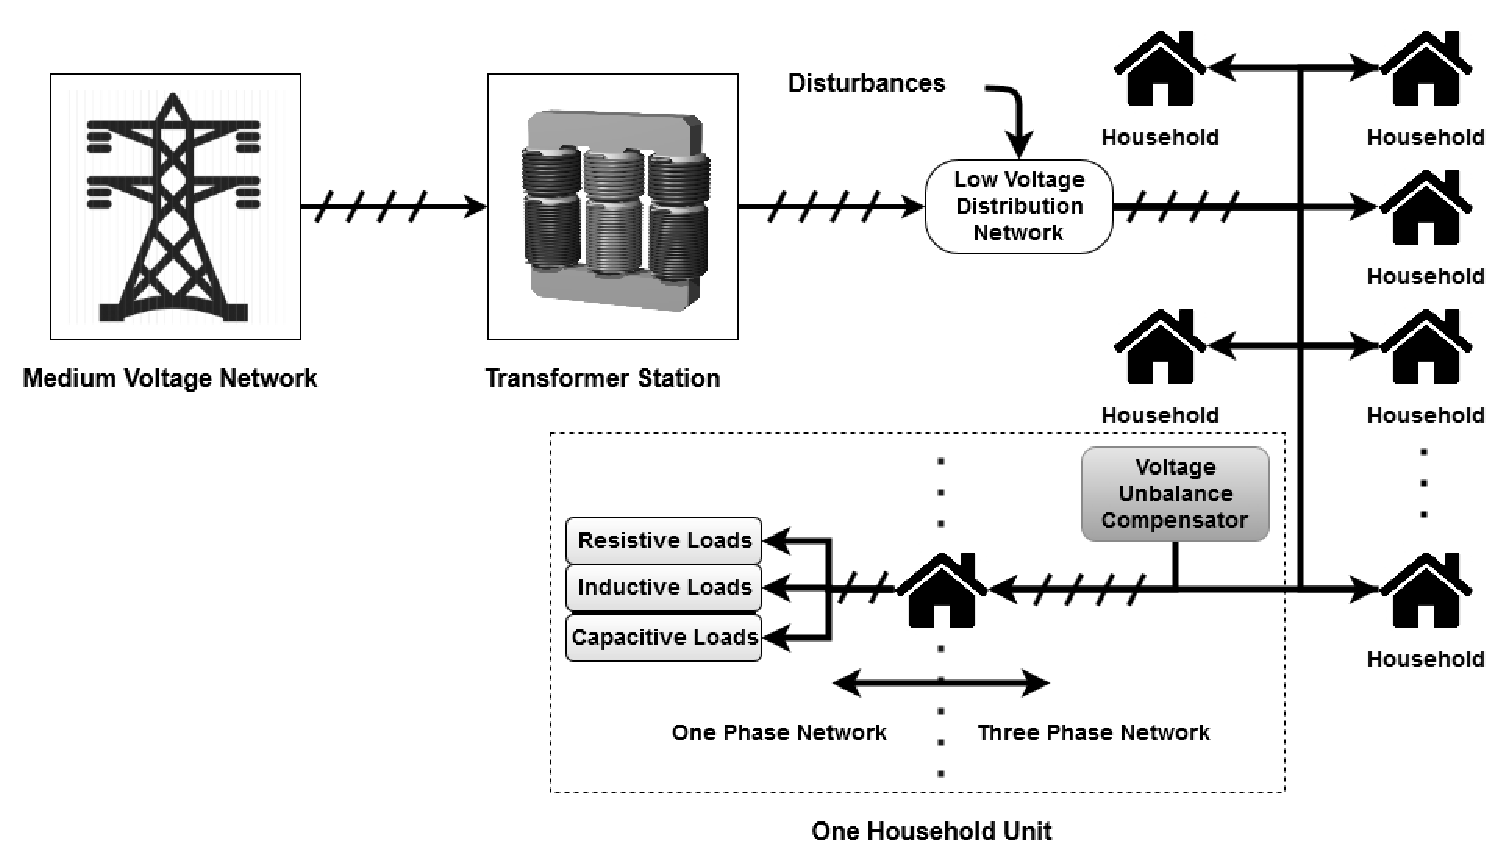
\includegraphics[width=\textwidth]{Unblance_EPS_Pics/network_gray.eps}
%            \caption{The simplified structure of a three phase four wire low voltage network. The transformer station acts as transition from the medium voltage power grid to
%            the low voltage network. The several regular households are representing the main loads of the network. The transformer and the loads are connected with power line sections infected by inductive and resistive disturbances and capacitive couplings. Domestic powerplants can connect to any connection point within the low voltage network, via an appropriate inverter - either to the three phase sections using a three phase inverter or to a single phase using a single phase inverter.}
%            \label{fig:network}
%            \end{figure}
%
%\subsubsection{Voltage unbalance}
%
%        There are many different technological causes of voltage unbalance with more or less practical importance. The following types of unbalance conditions are examined and tested in the sequel:
%        \begin{description}
%        \item[Single phase under-voltage unbalance]  If there is a single phase uncompensated overload in the system, the voltage in the overloaded phase will be lower than the other two.
%        \item[Two phase under-voltage unbalance]  Two of the three phases are overloaded without compensation, the two overloaded phases will have higher voltage drop than the third phase.
%        \item[Three phases under-voltage unbalance]  The loads of all three phases are overloaded in an unbalanced manner.
%        \item[Unequal single phase angle]  If the three phase voltage amplitudes are balanced but the relative angles between them (ideally it should be equal to $\pm120$ degree). It is assumed, that phase A would be the reference. If one of the other two phase angles is deflected, unequal displacement.
%        \item[Unequal two phase angles displacement] Similar to the single phase angle unbalance, if the other two phase angles are both deflected, then unequal angle displacement in two phase angles occurs.
%        \end{description}
%        An indicator of the voltage unbalance is supposed to measure the extent of unbalance but it is not expected to classify between the above types.
%
%        \paragraph{Standard indicators of unbalance}
%
%            Although the term voltage unbalance is unambiguous, the root phenomenon may be various as well as the standard norms used to measure unbalance. All of these different indicators measure voltage unbalance but each of them does it in a different way (\ref{equ:regular}).
%
%            \begin{eqnarray}
%              IEEEv_{936}&=&\frac{\max\{V_{an},V_{bn},V_{cn}\}-\min\{V_{an},V_{bn},V_{cn}\}}{\textnormal{mean}\{V_{an},V_{bn},V_{cn}\}}\times100\\
%              IEEEv_{112}&=&\frac{\textnormal{max deviation from mean of}\{V_{an},V_{bn},V_{cn}\}}{\textnormal{mean}\{V_{an},V_{bn},V_{cn}\}}\times100\\
%              MDV&=&\frac{\textnormal{max deviation from mean of}\{V_{ab},V_{bc},V_{ca}\}}{\textnormal{mean}\{V_{ab},V_{bc},V_{ca}\}}\times100\\
%              VUF&=&\frac{\textnormal{negative seq.voltage}}{\textnormal{positive seq.voltage}}\times100
%              \label{equ:regular}
%              \end{eqnarray}
%
%            The voltages $\{V_{an},V_{bn},V_{cn}\}$ denotes the phase-to-neutral voltages, while $\{V_{ab},V_{bc},V_{ca}\}$ are the line-to-line voltages, $V_1$ is equal to the voltage amplitude of the fundamental frequency and $V_n$ is the voltage amplitude of the $n$-th upper harmonic voltage \cite{bina2011three}  (current unbalance formulations are simply obtained by replacing voltage with current components). Although the harmonic distortion does not relate closely to the asymmetry phenomenon, it might cause a variety of problems like dropping efficiency of electric motors.
%
%            The above four norms measure different values for a single case. The first two standard indicators, $V_{936}$ and $V_{112}$, ignore the $\pm120$ degree phase difference unbalance and only take the amplitudes into account. The last two definitions, $MDV$ and $VUF$, are sensitive to the phase difference unbalance. Nevertheless, these definitions ignore zero sequence components and harmonic distortion that are always present in three-phase four-wire systems \cite{bina2011three}.
%
%         \subsubsection{Proposed vectorial indicator of unbalance}
%
%             Motivated by the deficiencies of standard voltage unbalance indcators (\ref{equ:regular}) the first problem is to find novel norm like indicators of unbalance that perform better, e.g. takes zero sequence voltages into account. One possible direction is motivated by vector calculus (see Figure \ref{fig:Vect}). The norm $N$ is defined as follows:
%
%             \begin{equation}
%                 \begin{array}{rcl}
%                     \Delta R&=&230e^{j0}-V_{an}\\
%                     \Delta S&=&230e^{j120}-V_{bn}\\
%                     \Delta T&=&230e^{j240}-V_{cn}\\
%                     N&=&|\Delta R\,\Delta S|+|\Delta R\,\Delta T|+|\Delta S\,\Delta T|\\
%                 \end{array}
%                 \label{equ:vect}
%             \end{equation}
%
%             where $\Delta R$, $\Delta S$,and $\Delta T$ are the vectorial error of each phase, and $N$ is the absolute value of the cross products of the error vectors (Figure \ref{fig:Vect}). The two main advantage of this method are the fact that all forms of differences are taken into account, and computational simplicity.
%%
%%                 \begin{figure}
%%             \centering
%%             \includegraphics{UnbalRedComp_JCP-figure0.pdf}
%% %             \begin{tikzpicture}[thick,scale=1,draw opacity=1]
%% %             \begin{polaraxis}
%% %             \addplot[black,->,dotted,thick] coordinates {(0,0)(0,230) };
%% %             \addlegendentry{\small{Ideal phasors}}
%% %             \addplot[black,->,dashed,thick] coordinates {(0,0)(0,210) };
%% %             \addlegendentry{\small{Real phasors}}
%% %             \addplot[black,->,thick] coordinates {(0,210)  (0,230) };
%% %             \addlegendentry{\small{Ideal-Real difference}}
%% %             \addplot[black,->,dotted,thick] coordinates {(0,0)(120,230) };
%% %             \addplot[black,->,dotted,thick] coordinates {(0,0)(240,230) };
%% %             \addplot[black,->,dashed,thick] coordinates {(0,0)(125,210) };
%% %             \addplot[black,->,dashed,thick] coordinates {(0,0)(232,215) };
%% %             \addplot[black,->,thick] coordinates {(125,210) (120,230) };
%% %             \addplot[black,->,thick] coordinates {(232,215) (240,230) };
%% %             \end{polaraxis}
%% %             \end{tikzpicture}
%%             \caption{Vectorial norm based difference of a real asymmetric tree phase voltage and the ideal symmetric three phase phasors.}
%%             \label{fig:Vect}
%%             \end{figure}
%
%        %\paragraph{Proposed geometrical indicator of unbalance}
%
%            It can be stated that every difference between the ideal and the measured voltage in both amplitude phase and sub-harmonics causing a form of asymmetry. The problem can also be investigated from a geometrical point of view as it is depicted in Figure \ref{fig:threephase}. The three-phase voltage system's phasor diagram contains three  phase-to-neutral voltage vectors which can be regarded as the points of a triangle (similarly, the three line-to-line vectors can play the role of the edges of the triangle). The two triangles (i.e. the ideal and the actual ones) always intersect except from very extreme and physically meaningless cases. The area where the two triangles do not cover each other (i.e. the difference of their union and intersection) can be used as a norm of voltage unbalance. In fact it is computationally more demanding compared to the previous methods, but takes every deviation into consideration \cite{Neukirchner2015},\cite{neukirchner2015examination}. The calculation of asymmetry error is given by (\ref{equ:geom}).
%            \begin{equation}
%                \begin{array}{rcl}
%                       G&=&\textnormal{Area of }(\bigtriangleup_{Ideal}\cup\bigtriangleup_{Real}-\bigtriangleup_{Ideal}\cap\bigtriangleup_{Real}),
%                \end{array}
%                \label{equ:geom}
%            \end{equation}
%            $\bigtriangleup_{Ideal}$ indicates the triangle spanned by the ideal voltage vectors and $\bigtriangleup_{Real}$ the triangle of real voltage vectors. Difference of the ideal and the real triangle's union and intersection defines the norm $G$.
%
%            \begin{figure}[!ht]
%           \centering
%           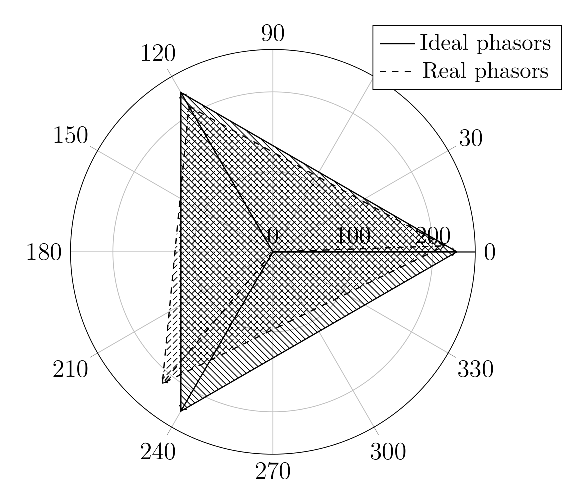
\includegraphics[scale=0.95]{Unblance_EPS_Pics/UnbalRedComp_JCP-figure1.eps}
%%                \begin{tikzpicture}[thick,scale=1,draw opacity=1]
%%                tick label style = {font=\sansmath\sffamily},
%%                every axis label = {font=\sansmath\sffamily},
%%                legend style = {font=\sansmath\sffamily},
%%                label style = {font=\sansmath\sffamily}
%%
%%                    \begin{polaraxis}%[nodes near coords,enlargelimits=0.2]
%%                    \addplot[pattern=north west lines,semithick] coordinates {(0,230) [A] (120,230) [B] (240,230) [C] (0,230)};
%%                    \addlegendentry{\small{Ideal phasors}}
%%
%%                    \addplot[pattern=north east lines,dashed,semithick,fill opacity=.3] coordinates {(2,215) ( 120,210) (230,215) (2,215)};
%%
%%                    %\addplot[orange] fill between[of=A and B];
%%                    \addlegendentry{\small{Real phasors}}
%%
%%
%%                    \addplot[->,semithick] coordinates {(0,0)(0,230) };
%%                    \addplot[->,semithick] coordinates {(0,0)(120,230) };
%%                    \addplot[->,semithick] coordinates {(0,0)(240,230) };
%%                    \addplot[dashed,->,semithick] coordinates {(0,0)(2,215) };
%%                    \addplot[dashed,->,semithick] coordinates {(0,0)(120,210) };
%%                    \addplot[dashed,->,semithick] coordinates {(0,0)(230,215) };
%%
%%                    \end{polaraxis}
%%                \end{tikzpicture}
%
%           \caption{The triangles spanned by the ideal and the actual voltage phasors. The extent of voltage unbalance on the network can be measured by the sum of areas where the two triangles are not overlapping.}
%           \label{fig:threephase}
%            \end{figure}
%
%
%
